\ifx\wholebook\relax\else
\input{../Common.tex}
\input{../macroes.tex}
\begin{document}
\fi

\chapter{Combining Methods}\label{ch:composons}

\begin{chapterfigure}
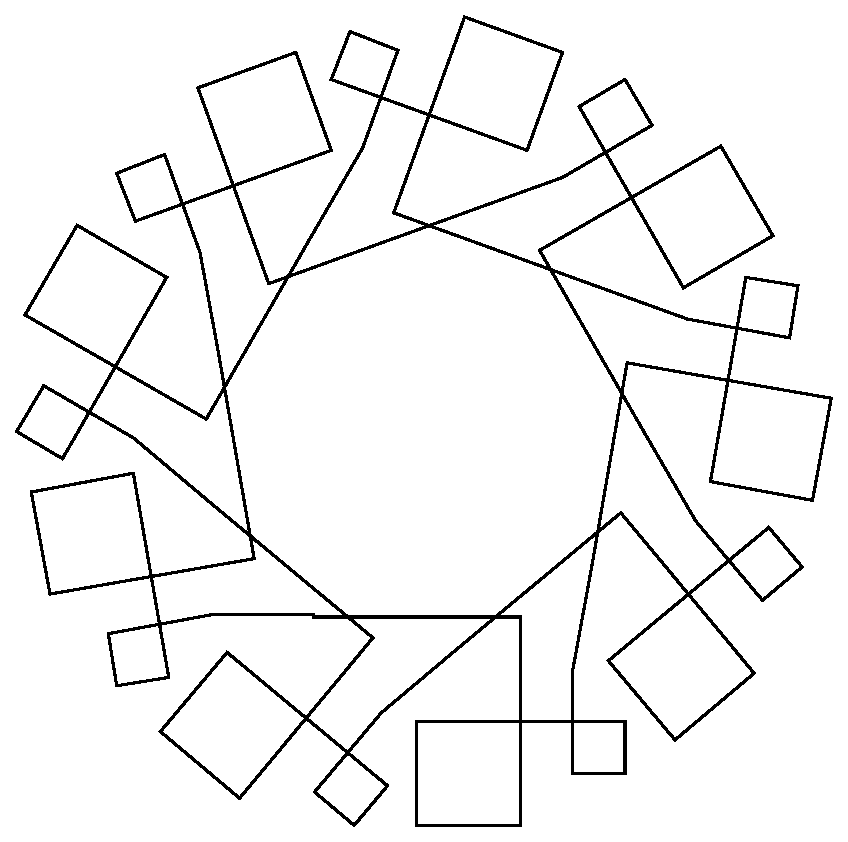
\includegraphics[width=6cm]{compArtNouveauTurningScr}
\end{chapterfigure}

In  Chapter~\ref{ch:turtleTeaching}, you learned how to define methods. I showed that defining methods is interesting because (1) methods avoid rewriting scripts and introducing errors and (2) methods can be used by different robots. The other main advantage of using methods  is the possibility of reusing methods, that is defining a method by calling other already existing methods. Reuse is what we will explore in this chapter.

Being able to reuse methods is extremely important because we can define a method in terms of another one, without having to know all the details of how the second method is defined.  We just call it.

\section{Nothing Really New: the \ct{square} Method}
Composing methods is quite natural and is not really new. Actually it is what we did in Chapter~\ref{ch:turtleTeaching} when you defined a method! The method \ct{square} is defined by calling the methods \turnLeft, \ct{go:} and \timesRepeat (as shown by method~\ref{comp:square}). Even \ct{square} is defined in terms of other methods, and we don't have to know how \turnLeft, \ct{go:} or \timesRepeat are defined. So we are already done with this chapter!

\begin{method}\label{comp:square}
\textbf{square}
   "Draw a square of 100 pixels wide "

   4 timesRepeat: 
         [ self go: 100;
                  turnLeft: 90 ]
\end{method}


\section{Other Graphical Patterns}
In Chapter~\ref{ch:turtleTeaching}, I asked you to define the method \ct{pattern} that draws a nice pattern (See~\scrref{src:artNouveau}). Now I ask you to perform  the experiment and produce the following drawings by defining more methods. 

%We remind you the definition of this method if you forgot to save it, so that you can define it now. 
%\begin{methodfig}{compArtNouveauScr}\label{src:mth:artnouveau}
%artNouveau
%   "draws a thing"

%   self go: 100.
%   self turnRight: 90.
%   self go: 100.
%   self turnRight: 90.
%   self go: 50.
%   self turnRight: 90.
%   self go: 50.
%   self turnRight: 90.
%   self go: 100.
%   self turnRight: 90.
%   self go: 25.
%   self turnRight: 90.
%   self go: 25.
%   self turnRight: 90.
%   self go: 50
%\end{methodfig}



\begin{exofigwithsize}[0.5]{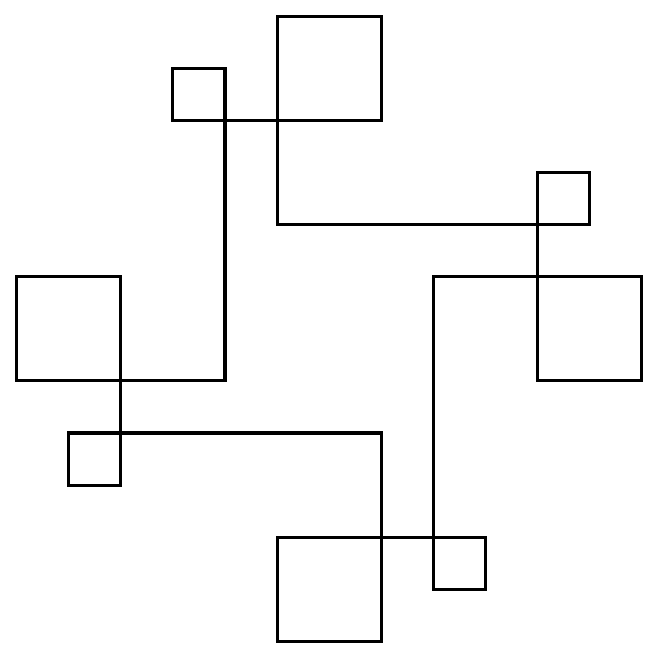
\includegraphics[width=5cm]{compCompleteThing}}
Define the method \ct{pattern4} that calls \ct{pattern} 4 times to produce the figure on the right. 
You will also use this method in another script later.

\begin{nalltt}
| \caro |
\caro := \Turtle new.
\caro pattern4
\end{nalltt}
\end{exofigwithsize}

\begin{exonofig}
Define the method \ct{tiltedPattern}  draws the picture at the beginning of this Chapter. Hint: you have to repeat the pattern 9 times, and the angle to turn is 10 degrees.

\end{exonofig}

\hidden{\begin{nalltt}
tiltedPattern 

   9 timesRepeat: 
                  [ self pattern. 
                  self turnRight: 10. 
                  self go: 50 ]
\end{nalltt}}


\begin{exofigwithsize}[0.5]{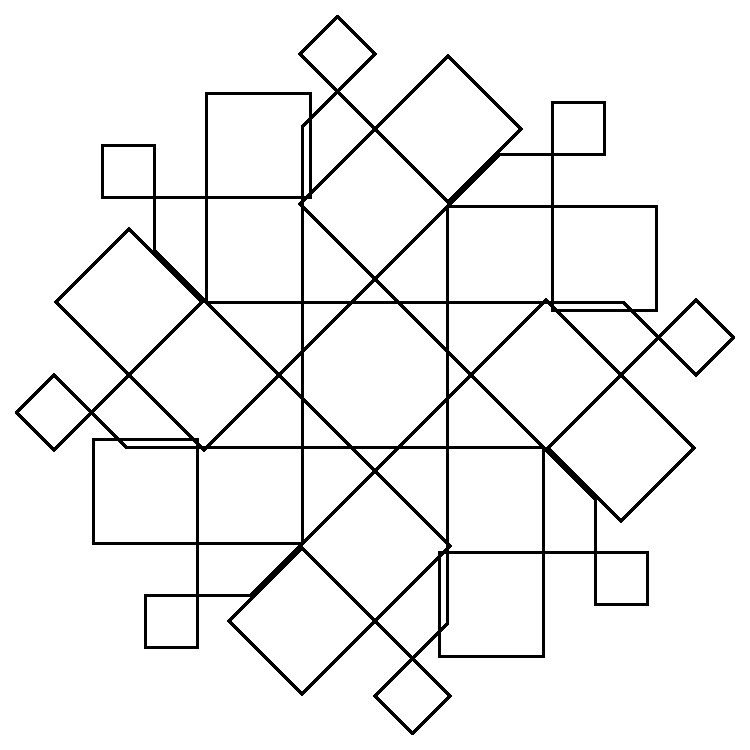
\includegraphics[width=6cm]{compArtNouveauGiantScr}}
Define the method \ct{doubleFrame} that draws the picture on the right. 

\

\begin{nalltt}
\textbf{doubleFrame}

    8 timesRepeat: 
                   [ self pattern. 
                   self turnLeft: 45.
                   self go: 100 ]
\end{nalltt}
\end{exofigwithsize}




\section{Stepping Back}
Now let's see what you can learn from the experiments you did. As you can see from the methods \ct{pattern4}, \ct{tiltedPattern}, and \ct{doubleFrame}, the method \ct{pattern} is only defined once, and then \emph{reused several times} in different methods. Defining \ct{pattern} as a method allows you to: (1) define it only once, (2) reuse it in various contexts and (3) not introduce errors during the rewriting of this method. 

If you look at the definition of the method \ct{doubleFrame}, you see that it is defined in terms of the \ct{pattern} method that is itself defined in terms of other methods such as \go, \turnLeft ... and so on. In fact, a complex method is often defined in terms of simpler methods, which themselves are defined in terms of even simpler methods --- and so on. This is because it is easier to understand and to define simpler methods.  In Chapter~\ref{ch:recomposing} I will show you that to solve a problem it is simpler to decompose it into smaller subproblems, solve them and then use the solution to smaller subproblems to finally solve the first problem. 

It is essential to understand that while defining the method \ct{doubleFrame} we do not have to know how \ct{pattern} is defined, we just need to know what it does and how to use it!  When we define a method we are giving a name to a sequence of messages, which reduces the number of details that we have to remember.  We just have to remember what the method does and its name, not how it does it.  We say that we are building an \emph{abstraction} over the definition details.

To make this point clear, I rewrote the method \ct{doubleFrame} without calling the method \ct{pattern} by directly copying the definition of \ct{pattern} (shown in italic) inside the other one. Compare \ct{doubleFrameWithoutCallingPattern} (method~\ref{mth:doubleFrameWithoutCallingPattern}) with the method \ct{doubleFrame}. The new version without \ct{pattern} is not only longer --- for most people it is also more confusing and harder to understand. 

Now imagine what would happen if I did the same with the code of \turnRight, \turnLeft, and \go --- because these are methods too. It would be a nightmare! There would be so many details that we would be lost all the time. 

\begin{method}\label{mth:doubleFrameWithoutCallingPattern}
\textbf{doubleFrameWithoutCallingPattern}

   8 timesRepeat: 
                  [ \textit{self go: 100.
                  self turnRight: 90.
                  self go: 100.
                  self turnRight: 90.
                  self go: 50.
                  self turnRight: 90.
                  self go: 50.
                  self turnRight: 90.
                  self go: 100.
                  self turnRight: 90.
                  self go: 25.
                  self turnRight: 90.
                  self go: 25.
                  self turnRight: 90.
                  self go: 50.}
                  self turnLeft: 45. 
                  self go: 100 ]
\end{method}



\largecadre{When you write a new method, it can call other methods.
You can use a method without knowing how it is written.
After you finish writing a method, you can call it when you write another method.}

\section{Squares Everywhere}
Now it is time to practice. Define the following methods using the method \ct{square}.


\begin{exonofig}{\textbf{Some Boxes.}}
Define the methods \ct{box} and \ct{separatedBox} that produce the 
pictures shown in Figure~\ref{c7groscarre}.
\end{exonofig}

\begin{figure}[h]
\begin{minipage}[c]{.30\linewidth}
\centerline{\includegraphics[width=4cm]{comp4Squares}}
\end{minipage}
\hfill
\begin{minipage}[c]{.30\linewidth}
\centerline{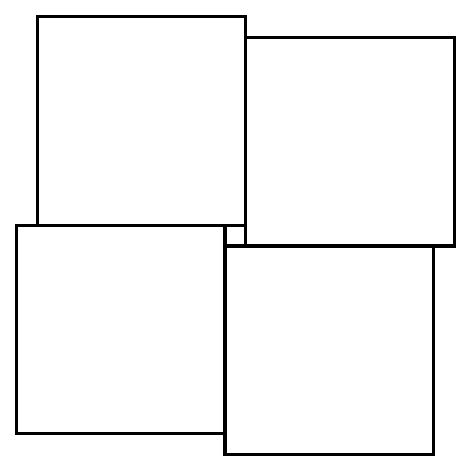
\includegraphics[width=4cm]{comp4SquaresTwo}}
\end{minipage}
\label{c7groscarre}
\end{figure}
 

\hidden{
| caro |
caro := Turtle new.
4 timesRepeat: [caro square100.
               caro turnLeft: 90]

| caro |
	caro := Turtle new.
	4 timesRepeat: 
		[ caro compSquareL100.
        caro turnLeft: 90. 
		caro go: 10]
}

\begin{exonofig}
Using your previous methods to generate various figures.
\end{exonofig}

\hidden{
\begin{alltt}
| caro |
caro := Turtle new.
12 timesRepeat: [caro square100.
                caro turnLeft: 30.
                caro go: 10]
\end{alltt}}


\begin{exonofig}{\textbf{Star.}} 
Using the method \ct{box}, experiment and define a method \ct{star} that produces the right-hand picture in Figure~\ref{c7star}.
\end{exonofig}

\begin{figure}[h]
\begin{minipage}[c]{.4\linewidth}
\centerline{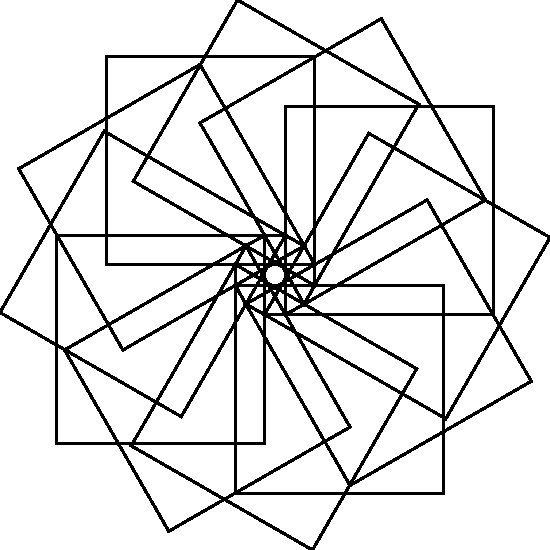
\includegraphics[width=4cm]{comp4SquaresThree}}
\end{minipage}
\hfill
\begin{minipage}[c]{.4\linewidth}
\centerline{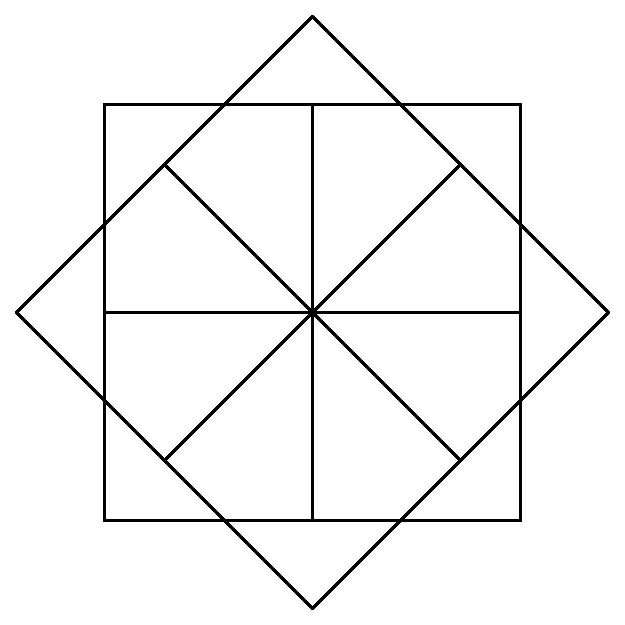
\includegraphics[width=4cm]{comp4SquaresFour}}
\end{minipage}
\label{c7star}
\caption{Stars}
\end{figure}


\summa

When you write a new method, it can call other methods.
You can use a method without knowing how it is written.
After you finish writing a method, you can call it when you write another method.

\ifx\wholebook\relax\else
\end{document}\fi
